% !TEX program = xelatex
\documentclass[times,specification,annotation]{../common/itmo-student-thesis}

%% Опции пакета:
%% - specification - если есть, генерируется задание, иначе не генерируется
%% - annotation - если есть, генерируется аннотация, иначе не генерируется
%% - times - делает все шрифтом Times New Roman, собирается с помощью xelatex
%% - languages={...} - устанавливает перечень используемых языков. По умолчанию это {english,russian}.
%%                     Последний из языков определяет текст основного документа.

\usepackage{icomma}
\usepackage{tabularx}
\usepackage{tikz}
\usetikzlibrary{arrows}

\addbibresource{bibliography/common.bib}
\addbibresource{bibliography/evolutionary.bib}
\addbibresource{bibliography/parallel.bib}
\addbibresource{bibliography/sat-usages.bib}
\addbibresource{bibliography/sequential.bib}
\graphicspath{ {../assets/} }

\begin{document}

\studygroup{M3439}
\title{Разработка параллельных алгоритмов решения задачи булевой выполнимости с использованием 
       поиска вероятностных лазеек}
\author{Джиблави Ибрагим Билалович}{Джиблави И.Б.}
\supervisor{Чивилихин Даниил Сергеевич}{Чивилихин Д.С.}{к.т.н.}{ординарный доцент}
\publishyear{2022}
\startdate{31}{января}{2022}
\finishdate{15}{мая}{2022}
\defencedate{15}{июня}{2022}

\secretary{Павлова О.Н.}

%% Задание
%% Техническое задание и исходные данные к работе
\technicalspec{Ключевой задачей является разработка эффективного алгоритма решения задач булевой
    выполнимости. Алгоритм по заданной формуле должен возвращать информацию о её
    выполнимости. Подразумевается параллельный алгоритм, использующий поиск
    вероятностных лазеек для сведения задачи к набору более простых подзадач и
    последующему решению этих подзадач с применением существующих решателей.}

%% Содержание выпускной квалификационной работы (перечень подлежащих разработке вопросов)
\plannedcontents{В данной работе разработаны алгоритмы поиска вероятностных лазеек на основе
    эволюционных алгоритмов. Разработаны различные подходы к решению на основе методов
    поиска вероятностных лазеек, исследована их эффективность. Проведено сравнение
    эффективности с существующими конкурентоспособными алгоритмами.}

%% Исходные материалы и пособия
\plannedsources{\begin{enumerate}
        \item TBD.
    \end{enumerate}}

%% Цель исследования
\researchaim{TBD}

%% Задачи, решаемые в ВКР
\researchtargets{\begin{enumerate}
        \item разработка эффективных алгоритмов поиска вероятностных лазеек.
        \item разработка методов решения задачи булевой выполнимости с применением вероятностных 
            лаззек.
        \item исследование эффективности полученных алгоритмов.
    \end{enumerate}}

%% Использование современных пакетов компьютерных программ и технологий
\addadvancedsoftware{Что}{Раздел работы}

%% Краткая характеристика полученных результатов
\researchsummary{TBD}

\researchfunding{TBD}

\researchpublications{TBD}

\maketitle{Бакалавр}

\tableofcontents

%&latex
\label{introduction}
\startprefacepage

Задача булевой выполнимости является крайне важной NP-полной~\cite{bib:cook-levin} алгоритмической
задачей, так как к ней сводится большое число задач. Среди них:
\begin{itemize}
    \item Проверка моделей, использующийся для формальной верификации параллельных систем с
        конечным числом состояний~\cite{bib:use-mc}.
    \item Восстановление секретного ключа в алгоритме RSA~\cite{bib:use-rsa}.
    \item Разложение булевых матриц~\cite{bib:use-bma}, часто применяемое в рекоммендательных
        системах.
    \item 0-1 задача о рюкзаке (широко известная задача класса NP).
    \item Многие задачи планирования, например, one shop scheduling~\cite{bib:use-ojs}, сводятся к SAT.
\end{itemize}

Для задачи булевой выполнимости, как и для любой NP-полной задачи пока не известно алгоритма,
решающего её за полиномиальное от размера входа время. Однако, спектр применения этой задачи
достаточно широк, чтобы возникала практическая польза от разработки эффективных решателей.

Алгоритмы решения задачи булевой выполнимости глобально делятся на две категории. Первая --- 
последовательные решатели, то есть работающие в одном потоке исполнения. Существующие эффективные
и широко распостраненные подходы к построению таких решателей более подробно описаны в Главе~
\ref{overview:sequential}. Вторая --- параллельные решатели, нацеленные на максимальную утилизацию доступных
ресурсов многоядерных и многопроцессорных машин для ускорения процесса решения. Более подробно
они описаны в Главе~\ref{overview:parallel}.

Целью данной работы является построение эффективного параллельного алгоритма решения задачи булевой
выполнимости на основе поиска вероятностных лазеек. В рамках исследований в TBD-REF данное семейство
подходов показало положительные результаты, однако остается достаточно большое пространство как для
построения более конкурентноспособной реализации, так и для расширения семейства подходов.

В рамках данной работы поставлены и выполнены следующие задачи:
\begin{itemize}
    \item Разработка эффективного алгоритма поиска вероятностных лазеек на основе подходов,
        изложенных в TBD-REF.
    \item Адаптация набора существующих решателей для использования в рамках разрабатываемых
        алгоритмов.
    \item Разработка альтернативных предложенным в TBD-REF схем решения с использованием
        вероятностных лазеек.
    \item Исследование эффективности реализованных схем и сравнение с существующими
        паралелльными решателями.
\end{itemize}

В Главе~\ref{overview:terms} содержатся необходимые понятия и определения. В 
Главе~\ref{overview:sequential} поверхностно рассмотрены существующие эффективные и широко
распостраненные подходы к реализации последовательных решателей. В Главе~\ref{overview:parallel}
более подробно описаны популярные и успешные стратегии работы параллельных решателей.

В Главе~\ref{arch:rbs} рассмотрен вопрос поиска вероятностных лазеек. В разделе~\ref{arch:rbs:schema}
построены эффективные эволюционные алгоритмы для решения этой задачи. В разделе~\ref{arch:rbs:prop}
описаны изменения, внесенные в исходный код Minisat, позволяющие существенно ускорить процесс поиска решения.
В Главе~\ref{arch:solver} описан построенный параллельный сервис для решения задач булевой
выполнимости. Описан процесс адаптации и унификации существующих последовательных решателей,
способы обмена знаниями между решателями.
В Главе~\ref{arch:solve} приведено описание и описана реализация как упоминаемых в TBD-REF,
так и новых стратегий использования вероятностных лазеек в решателе.

%\printannobibliography


%&latex
\chapter{Обзор}\label{overview}

\section{Термины и понятия}\label{overview:terms}

\begin{definition}\label{overview:formula}
    \textbf{Булевой формулой} \footnote{https://ru.wikipedia.org/wiki/Булева\_формула} называется 
    формула логики высказываний, сорержащая логические переменные и пропозициональные связки
    $\wedge, \vee, \neg$. Множество логических переменных обозначается $V$.
\end{definition}

\begin{definition}
    \textbf{Булевой функцией} называется отображение $E\colon~ \mathcal{B}^n \to \mathcal{B}$,
    где $\mathcal{B} = \{\, 0, 1 \,\}$, а $n$ -- число различных переменных. Булева формула $F$ 
    задает булеву функцию $E_F$. Далее разница между этими понятиями для нас несущественна, поэтому
    всегда будет упоминаться булева функция $E$.
\end{definition}

\begin{definition}
    \textbf{Задача булевой выполнимости (SAT)} --- проверить, существует ли $x \in \mathcal{B}$
    такой, что выполняется $E(x) = 1$.
\end{definition}

\begin{theorem}(Кук, Левин)~\cite{bib:cook-levin}
    \textit{Задача булевой выполнимости принадлежит классу NP-полных задач.}
\end{theorem}

\begin{definition}
    \textbf{Решателем, алгоритмом A} называется алгоритм, принимающий на вход описание булевой формулы $C$
    и выдающий результат проверки булевой выполнимости соответствующей булевой функции --- $A(C)$.
    Возможны следующие результаты:
    \begin{itemize}
        \item \texttt{0}, функция невыполнима.
        \item \texttt{1}, функция выполнима. В этом случае также может быть возвращено
            удовлетворяющее функции назначение переменных $R$: $E(V \mid R) = 1$.
        \item \texttt{?}, решатель не смог решить задачу либо вследствие его неполноты, либо
            из-за нехватки ресурсов, таких как время или память.
    \end{itemize}
    Обозначим за $S(A)$ множество булевых функций, разрешимых алгоритмом $A$ за полиномиальное время.
\end{definition}

\begin{definition}
    \textbf{Означиванием, подстановкой} набора переменных $B \subseteq V$ называется отображение
    $\hat{b}\colon~ B \to \mathcal{B}$. Означивание можно применить к булевой функции $E$,
    результатом будет другая булева функция $E[B \mid \hat{b}] \colon \mathcal{B}^{|V| - |B|} \to
    \mathcal{B}$, возможно тождественная. Она получается из исходной путем частичной подстановки
    переменных, назначенных функцией $\hat{b}$. Множество всех означиваний множества переменных
    $B$ обозначается $\hat{B}$.
\end{definition}

\begin{definition}
    \textbf{Лазейкой} называется множество $B \subseteq V$ такое, что для любого из $2^{|B|}$
    означиваний $\hat{b}$ переменных из $B$ выполняется $E[B \mid \hat{b}] \equiv 0$.
    Ясно, что если для функции $E$ существует лазейка, то она невыполнима, то есть $E \equiv 0$.
\end{definition}


\begin{definition}\label{overview:rho-backdoor}
    \textbf{$\rho$-Лазейкой} называется множество $B \subseteq V$ такое, что выполняется
\[
    \left|\left\{\, \hat{b} \mid \hat{b} \in \hat{B},~ E[B \mid \hat{b}] \equiv 0 \,\right\}\right|
    \geqslant \rho \cdot 2^{|B|}.
\]
\end{definition}

\newcommand*{\prob}{\mathsf{Pr}}

\begin{definition}\label{overview:prob-backdoor}
    \textbf{$(\varepsilon, \delta)$ аппроксимация лазейки, вероятностная лазейка}. Зафиксируем
    $\varepsilon, \delta \in (0, 1)$, пожмножество переменных $B \subseteq V$ и алгоритм $A$, 
    и рассмотрим множество означиваний $\hat{B}$ в терминах $\rho$-лазейки.
    \begin{itemize}
        \item Введем на $\hat{B}$ равномерное распределение и зададим случайную величину
            \[
                \xi_B(\hat{b}) = \left[E[B \mid \hat{b}] \in S(A)\right].
            \]
            Ясно, что эта величина распределена по Бернулли с $p = \rho_B$.
        \item Тогда $B$ является $(\varepsilon, \delta)$ аппроксимацией лазейки, если
            \[
                \prob{\left[1 - \varepsilon \leqslant \frac{1}{N}\sum_{j=1}^{N}{\xi_j}\right]}
                \geqslant 1 - \delta,
            \]
            где $N \geqslant \frac{4 \ln{2/\delta}}{\varepsilon^2}$. Данное условие согласно
            теореме Чернова TBD-REF обеспечивает тот факт, что аппроксимация $\rho_B$, 
            вычисляемая по формуле 
            \begin{equation}
                \hat{\rho}_B = \frac{1}{N} \sum_{j=1}^{N}{\xi_j}\label{overview:rho-hat},
            \end{equation}
            отклоняется от истинного значения $\rho_B$ не более, чем на $\varepsilon$ с вероятностью 
            не менее $1 - \delta$.
    \end{itemize}
\end{definition}

\startrelatedwork

\section{Последовательные решатели}\label{overview:sequential}

\section{Параллельные решатели}\label{overview:parallel}

\finishrelatedwork

\chapterconclusion


\chapter{Теоретическое исследование и архитектура}\label{arch}

\section{Поиск вероятностных лазеек}\label{arch:rbs}

\subsection{Схема алгоритма}\label{arch:rbs:schema}

В данной главе описаны алгоритмы поиска вероятностных лазеек.
Для поиска вероятностных лазеек применяются эволюционные алгоритмы, а именно, (1 + 1) и (q + h)
алгоритмы~\cite{bib:ea},~\cite{bib:ga}. Для полного описания теоретической схемы поиска 
вероятностных лазеек необходимо определить особь, фитнес-функцию, а также операторы скрещивания, 
мутации и отбора.

\textbf{Особью} во всех реализованных схемах поиска вероятностных лазеек является битовая маска
$\overline{B}$, соответствующая множеству переменных $B$, включенных в лазейку.

\textbf{Фитнес функция}. В фитнес-функции используется аппроксимация значения $\rho$, формально 
определенная уравнением \ref{overview:rho-hat}, так как такой
подход позволяет вычислять его с достаточно высокой точностью, а главное --- быстро. В качестве
алгоритма $A$ используется \textit{вывод последствий, или unit propagation (UP)}, эффективно реализованный
в рамках решателя Minisat~\cite{bib:minisat}. Данный алгоритм с точки зрения решателя не является
полным, но имеет полиномиальное время работы.

Используется фитнес функция, описанная в TBD-REF. Её преимущество заключается в том, что она помимо 
максимизации $\hat{\rho}$-значения лазейки минимизирует её размер. Максимизация $\hat{\rho}$-значения 
достигается первой частью функции:
\[
    G_{C}\left(\overline{B}\right) = (1 - \hat{\rho}_B) \cdot 2^{\omega |V|},
\]
где $C$ --- формула \ref{overview:formula}, $V$ --- множество переменных в формуле, $w \in (0, 1]$
-- константа. Минимизация размера лазейки обеспечивается второй частью функции:
\[
    f_{C, \min{|B|}} = \hat{\rho}_B \cdot 2^{|B|}.
\]
Действительно, при относительно близких значениях $\rho$ большое влияние на функцию будет оказывать
размер лазейки $B$. Итоговая фитнес функция выглядит следующим образом:
\begin{equation}
    f_{C}\left(\overline{B}\right) = \hat{\rho}_B \cdot 2^{|B|} + (1 - \hat{\rho}_B) \cdot 2^{\omega |V|}.
    \label{arch:fitness}
\end{equation}

\textbf{Операторы}
В качестве основного оператора мутации был выбран зарекоммендовавший себя в TBD-REF оператор 
\textsc{Doerr}~\cite{bib:doerr}. В процессе разработки также использовался равномерный оператор
мутации, однако результаты, которые он показывал, стабильно хуже результатов \textsc{Doerr} на
всех примерах, поэтому он был отброшен, однако доступен в конфигурации. Реализованы операторы
одноточечного и двуточечного скрещивания. Генетический алгоритм $(\mu + \lambda)$ был
реализован аналогично схеме, предложенной в TBD-REF.

\subsection{Эффективный вывод последствий}\label{arch:rbs:prop}

Основным потребителем ресурсов в описанной схеме поиска вероятностных лазеек является алгоритм
вывода последствий, реализованный в Minisat~\cite{bib:minisat}. Поэтому оптимизация этого алгоритма
и разработка новых подходов является крайне важной задачей для достижения высокой производительности.

\textit{Выборка}\label{arch:rbs:prop:sampling}. Заметим, что для достаточно маленьких $B$ имеет
смысл производить полный перебор множества $\hat{B}$ при вычислении $\hat{\rho}$. Во-первых,
это обеспечит точное значение $\hat{\rho} = \rho$, во-вторых, реализация перебора всех подстановок
(то есть, перебора всех возможных назначений переменных из набора в $\mathcal{B}$, что эквивалентно
перебору всех чисел от $0$ до $2^{|B|} - 1$ в двоичной записи) точно будет работать не медленнее,
чем случайный перебор $2^{|B|}$ подстановок, так как не пользуется геренацией случайных чисел и
делает строго меньше операций засчет того, что не на каждом шаге модифицируются все значения подстановки.

Данное наблюдение создает необходимость в абстракции от типа выборки. Для этого был создан интерфейс
\textsc{Search}, а также следующие реализации:
\begin{itemize}
    \item \textsc{FullSearch} --- перебор всех возможных $\hat{b} \in \hat{B}$.
    \item \textsc{RandomSearch} --- перебор $N$ случайных подстановок из $\hat{B}$.
    \item \textsc{UniqueSearch} --- перебор $N$ уникальных случайных подстановок из $\hat{B}$.
    \item \textsc{CartesianSearch} --- перебор всех подстановок из декартового произведения
        нескольких наборов подстановок, необходимая для реализации некоторых стратегий 
        (см. Главу \ref{arch:solve}).
\end{itemize}

На рисунке \ref{arch:rbs:prop:search-img} представлена схема наследования интерфейса \textsc{Search}.
Далее в таблице \ref{arch:rbs:prop:search-def} описаны методы интерфейса.

\begin{figure}[H]
    \caption{Интерфейс \textsc{Search} и его реализации}
    \centering
    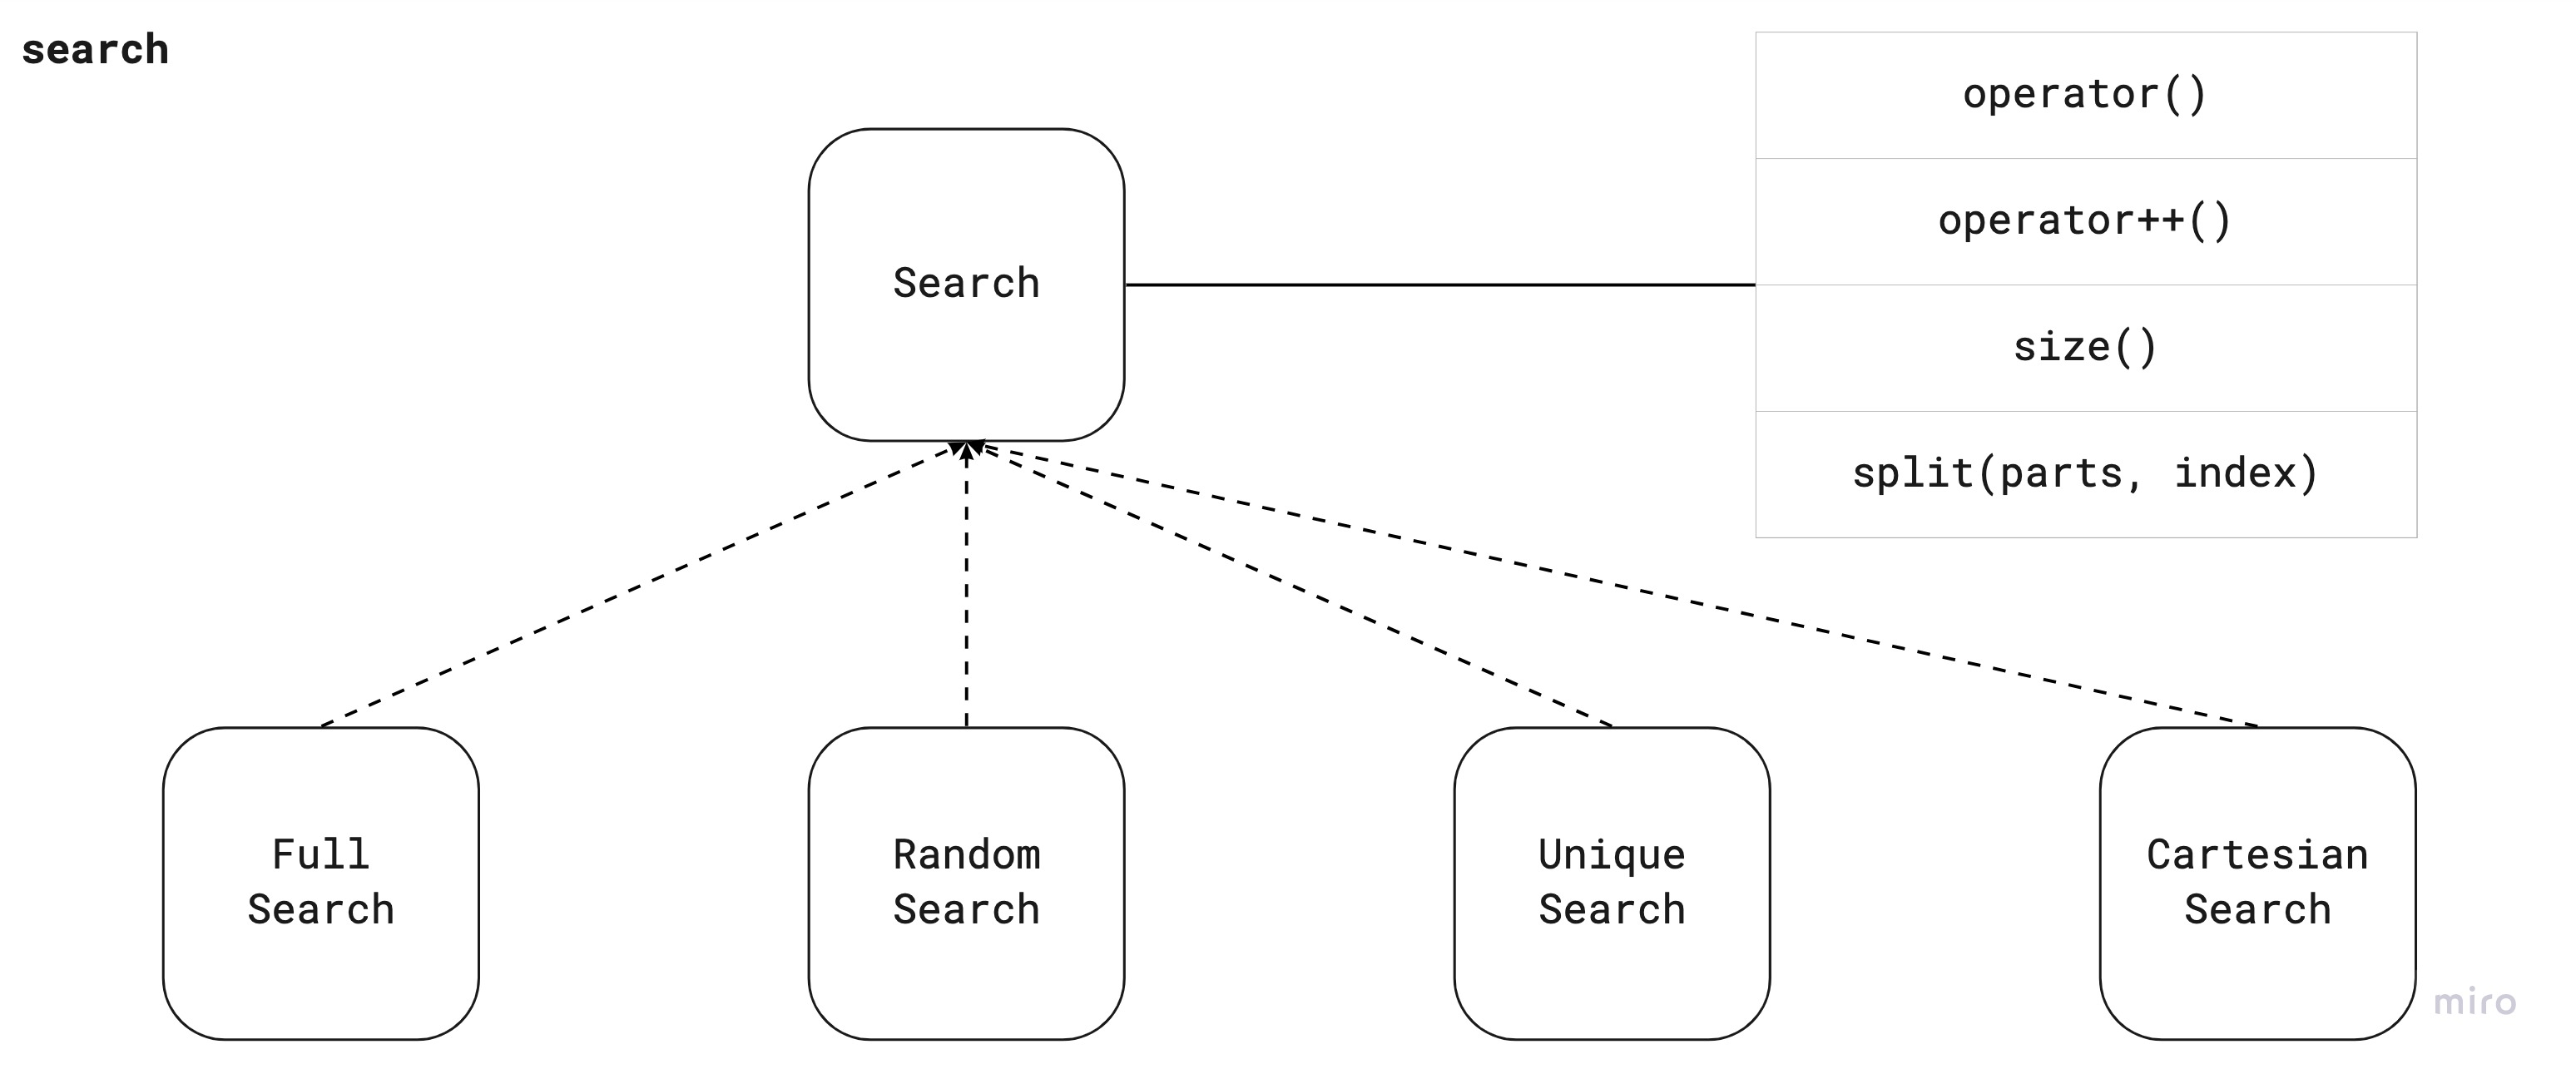
\includegraphics[width=\textwidth]{arch-search}
    \label{arch:rbs:prop:search-img}
\end{figure}

\begin{table}[H]
    \caption{Описание методов \textsc{Search}}\label{arch:rbs:prop:search-def}
    \centering
    \begin{tabularx}{\textwidth}{|*{3}{>{\centering\arraybackslash}X|}}\hline
        Метод & Параметры & Описание \\\hline
        \textsc{operator()} & -- & Возвращает текущий элемент выборки \\\hline
        \textsc{operator++} & -- & Переходит на следующий элемент выборки. Возвращает \textsc{false},
                                    если новый элемент -- последний \\\hline
        \textsc{size} & -- & Возвращает размер выборки \\\hline
        \textsc{split} & Число потоков, номер потока & Возвращает часть исходной выборки \\\hline
    \end{tabularx}
\end{table}

После получения выборки необходимо вызвать метод вывода последствий на всех элементах этой
выборки. Далее будут рассмотрены различные подходы к решению этой задачи: \textit{наивный
(последовательный), параллельный, вычисление $\rho$ через дерево поиска}.

\textit{Наивный подход}\label{arch:rbs:prop:naive}. Данный подход подразумевает последовательный
вызов метода вывода последствий. То есть, имея выборку $D$ и решатель $A$, значение $\rho$ 
аппроксимируется так, как показано в листинге \ref{arch:rbs:prop:naive-lst}.

\algdef{SE}[DOWHILE]{Do}{doWhile}{\algorithmicdo}[1]{\algorithmicwhile\ #1}%

\begin{algorithm}[H]
\caption{Наивное вычисление $\hat{\rho}$}\label{arch:rbs:prop:naive-lst}
\begin{algorithmic}
	\Function{calculate\_rho}{\textsc{A}, \textsc{D}}
        \State $S \leftarrow 0$
        \Do
            \State $\hat{b} \leftarrow \textsc{D()}$
            \If{\textsc{A($\hat{b}$)} = 0}
				\State $S \leftarrow S + 1$
			\EndIf
        \doWhile{\textsc{D++}}
        \State\Return $\frac{S}{N}$
	\EndFunction
\end{algorithmic}
\end{algorithm}

\textit{Параллельная обработка выборки}\label{arch:rbs:prop:par}. Данный подход разделяет выборку
на несколько выборок и обрабатывает их в разных потоках. Для этого используется метод \textsc{split}.
Псевдокод данного подхода представлен в листинге \ref{arch:rbs:prop:par-lst}.

\begin{algorithm}[H]
\caption{Параллельное вычисление $\hat{\rho}$}\label{arch:rbs:prop:par-lst}
\begin{algorithmic}
    \Function{calculate\_rho\_par}{$[\textsc{A}_i, i=\overline{1,M}]$, \textsc{D}}
        \State $S \leftarrow 0$
        \State $[\textsc{D}_i] \leftarrow \left[\textsc{D.split($M$, $j$),~ $j=\overline{1,M}$}\right]$
        \State\Return $\sum_{i}^{\textsc{parallel}}{\textsc{calculate\_rho($A_i$, $D_i$)}} / N$
	\EndFunction
\end{algorithmic}
\end{algorithm}

Данный подход с теоретической точки зрения крайне хорошо масштабируется, так как метод \textsc{split}
занимает несравнимо мало времени по сравнению с многократным вызовом метода вывода последствий. Практическое
сравнение последовательного и параллельного подходов приведено в Главе \ref{research:prop}.

\textit{Вычисление точного значения $\rho$ через дерево подстановок}\label{arch:rbs:prop:tree}.
Данный подход является новым и не имеет аналогов в известных мне решателях за ненадобностью. Однако,
идея, описанная далее, является крайне эффективной оптимизацией перебора $\hat{B}$, как показано в
Главе~\ref{research:prop}. Для вычисления точного значения $\rho$ необходимо посчитать число
подстановок $\hat{b} \in \hat{B}$, которые решаются заданным алгоритмом $A$. В данной работе, как
упомянуто ранее, в качестве этого алгоритма используется алгоритм вывода последствий. Результатом
работы этого алгоритма может быть либо информация о существовании конфликтующих подстановок переменных,
либо отсутствие дополнительной информации. Заметим, что если на каком-то префиксе $\hat{b}$ 
алгоритм сообщил о конфликте, то нет никакого смысла далее рассматривать подстановки с этим префиксом,
так как все они заведомо конфликтные. Можно просто прибавить к результату размер всего поддерева поиска.
Иллюстрация к данной идее приведена на рисунке \ref{arch:rbs:prop:tree-img}. Листинг, содержащий
псевдокод данного метода, приведен в приложении (листинг~\ref{append:rbs:prop:tree-lst}). Данный
метод был успешно реализован и встроен в исходный код решателя Minisat. Сравнительные результаты
с наивным и параллельным подходами содержатся в Главе~\ref{research:prop}.

\begin{figure}[H]
    \caption{Вычисление $\rho$ через дерево подстановок. Здесь $X,Y,Z$ --- переменные. Подстановки
    $E[X \mid 1]$ и $E[\{\,X,Y\,\} \mid \{\, X \to 0,~ Y \to 1 \,\}]$ приводят к конфликту, поэтому
    соответствующие поддеревья поиска можно не рассматривать.}
    \centering
    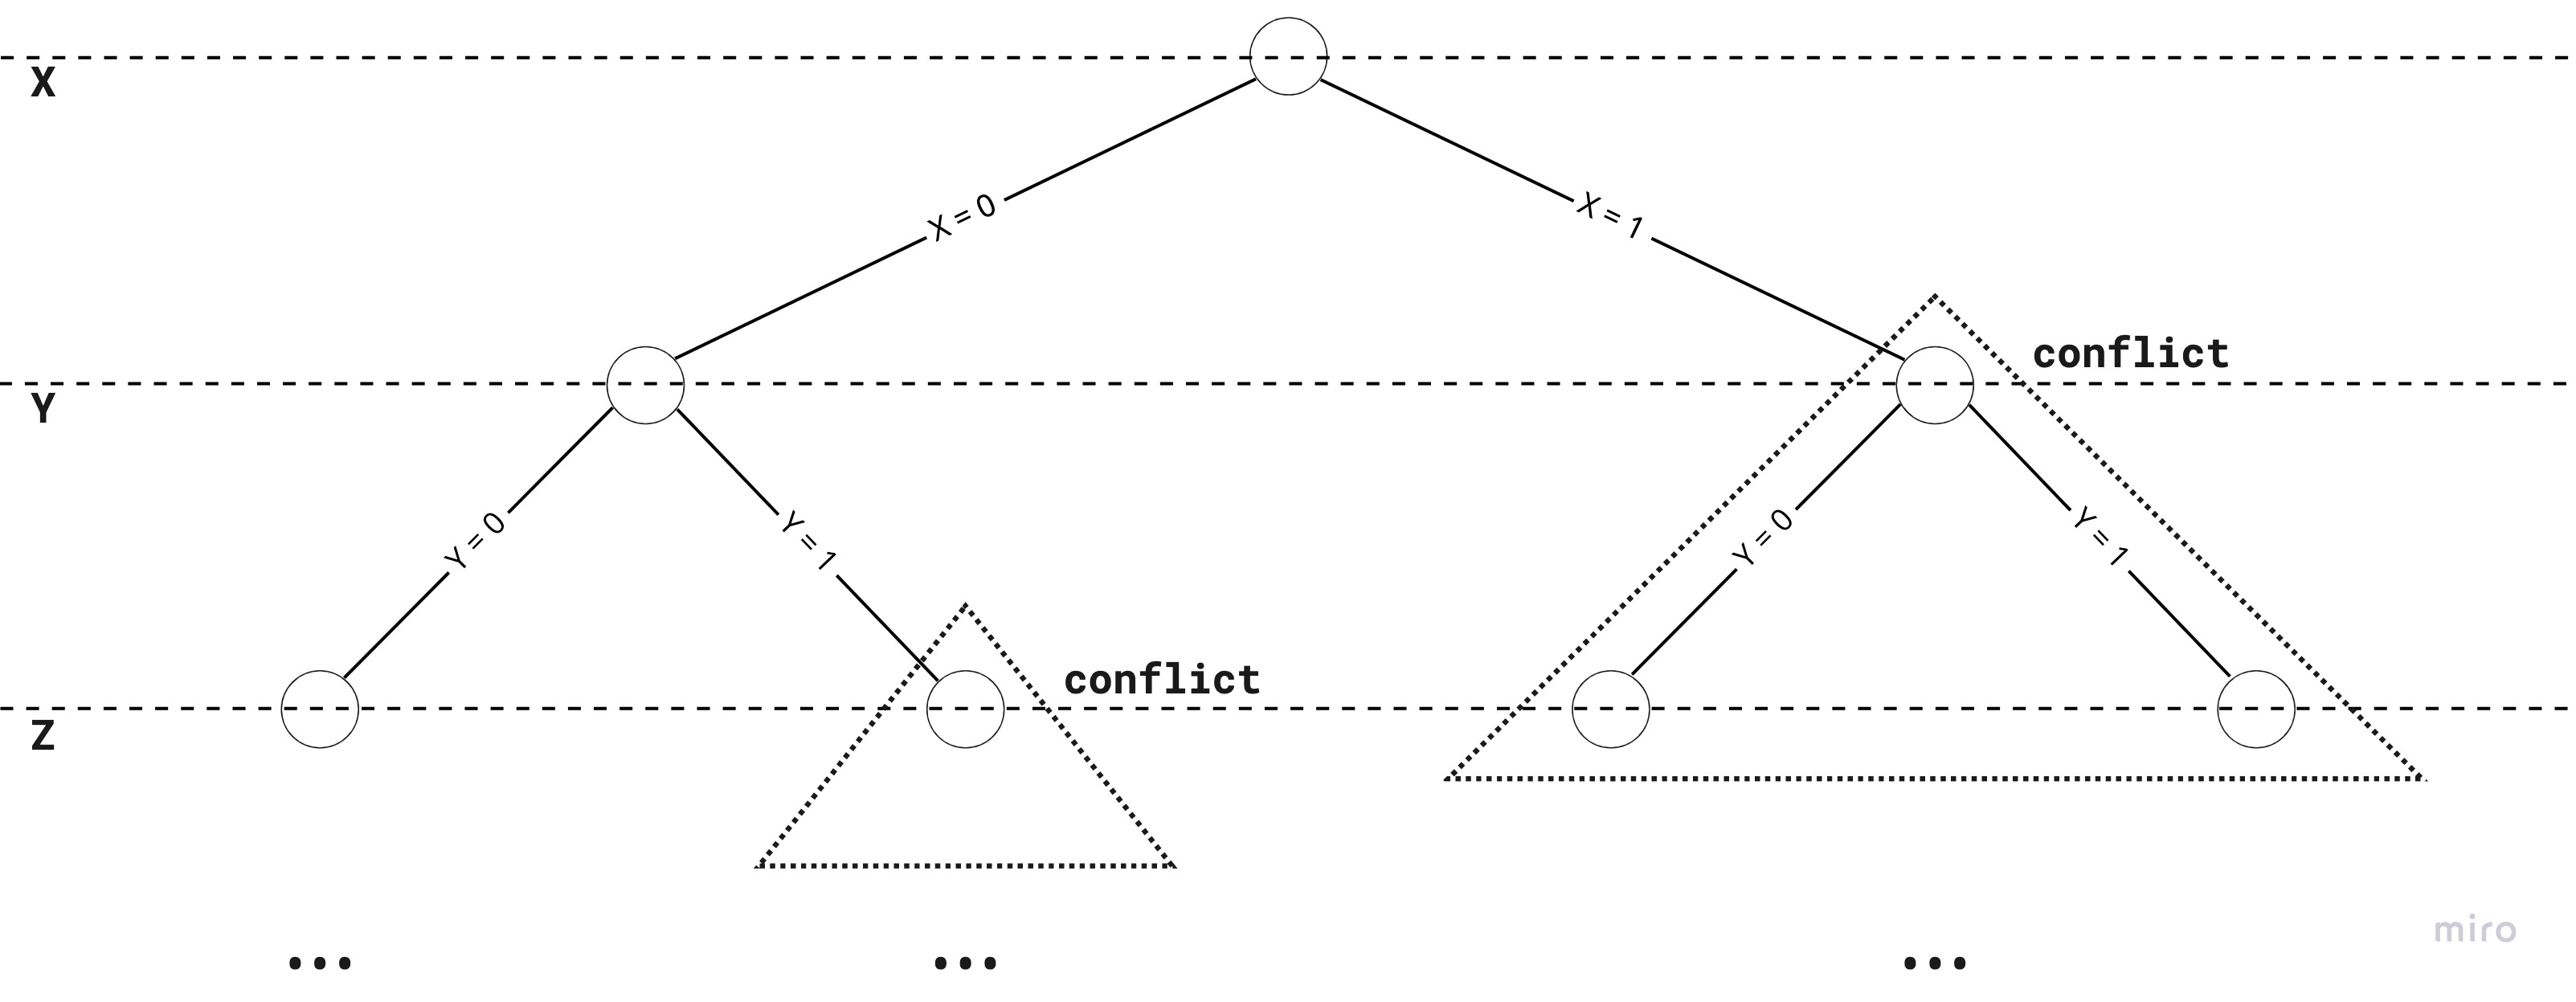
\includegraphics[width=\textwidth]{arch-tree}
    \label{arch:rbs:prop:tree-img}
\end{figure}

\section{Решение набора подстановок}\label{arch:solver}

В данной главе описана архитектура сервиса решения булевой функции с подстановками. Описан интерфейс
сервиса, приведена схема распределения задач по последовательным решателям, описана техника обмена
знаниями между решателями.

В качестве последовательных решателей используются Minisat~\cite{bib:minisat},
MapleCOMSPS~\cite{bib:maplecomsps}, painless-maplecomsps~\cite{bib:painless}. Под последовательным
имеется в виду не тип самого решателя, а невозможность параллельного решения разных задач.
То есть, painless-mcomsps является параллельным решателем, но может решать лишь одну задачу
одновременно. Описываемый сервис нужен именно для того, чтобы обеспечить возможность параллельного 
решения разных задач, что необходимо для реализации параллельных алгоритмов решения на основе 
подхода разделяй-и-властвуй~\ref{overview:dac}.

Схема наследования интерфейса \textsc{SolverService} проиллюстрирована на рисунке~\ref{arch:solver:serv-img}.
Описание методов интерфейса приведено в таблице~\ref{arch:solver:serv-def}.

\begin{figure}[H]
    \caption{Интерфейс \textsc{SolverService} и его реализация}
    \centering
    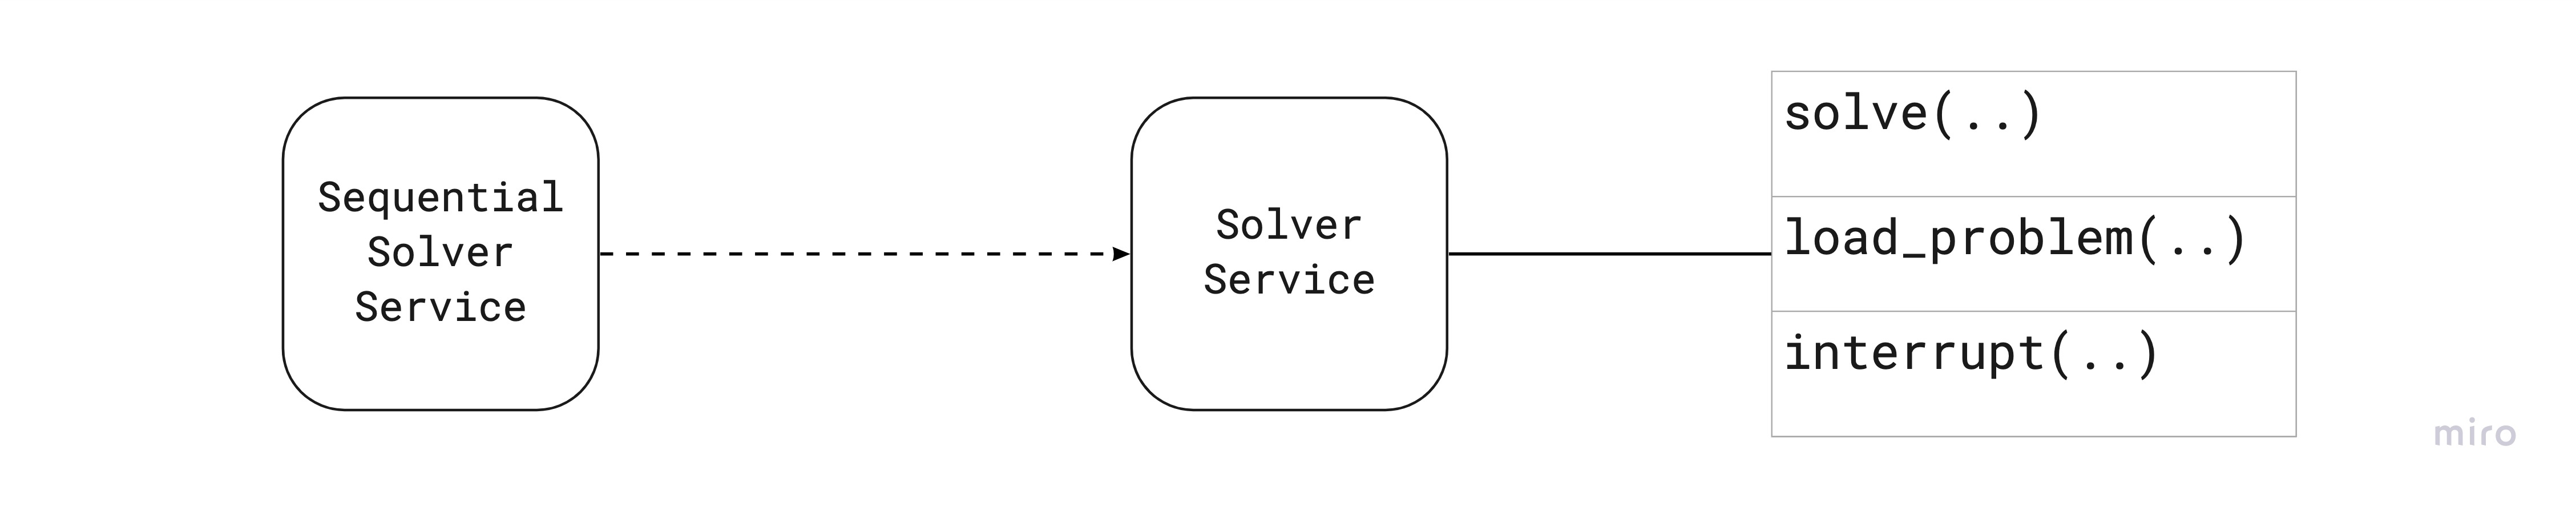
\includegraphics[width=\textwidth]{arch-solver}
    \label{arch:solver:serv-img}
\end{figure}

\begin{table}[H]
    \caption{Описание методов \textsc{SolverService}}\label{arch:solver:serv-def}
    \centering
    \begin{tabularx}{\textwidth}{|*{3}{>{\centering\arraybackslash}X|}}\hline
        Метод & Параметры & Описание \\\hline
        \textsc{solve} & Подстановка, ограничение по времени, callback-функция, вызываемая 
                        при окончании решения & Возвращает объект \textsc{std::future} типизированный
                        результатом решения, и добавляет задачу в очередь \\\hline
        \textsc{load\_problem} & -- & Загружает формулу в решатель \\\hline
        \textsc{interrupt} & -- & Прерывает процесс решения \\\hline
    \end{tabularx}
\end{table}

Реализация \textsc{SequentialSolverService} управляет набором последовательных решателей, работающих
параллельно: обеспечивает их задачами, а также, при необходимости, обеспечивает обмен знаниями.
Для распределения задач реализована безопасная для использования в многопоточной среде очередь.
Для обмена знаниями используются механизмы, реализованные в интерфейсе \textsc{painless} и адаптированные
для использования разных решателей и схем обмена. Схема работы \textsc{SequentialSolverService}
приведена на рисунке~\ref{arch:solver:seq-img}.

\begin{figure}[H]
    \caption{Схема работы \textsc{SequentialSolverService}}
    \centering
    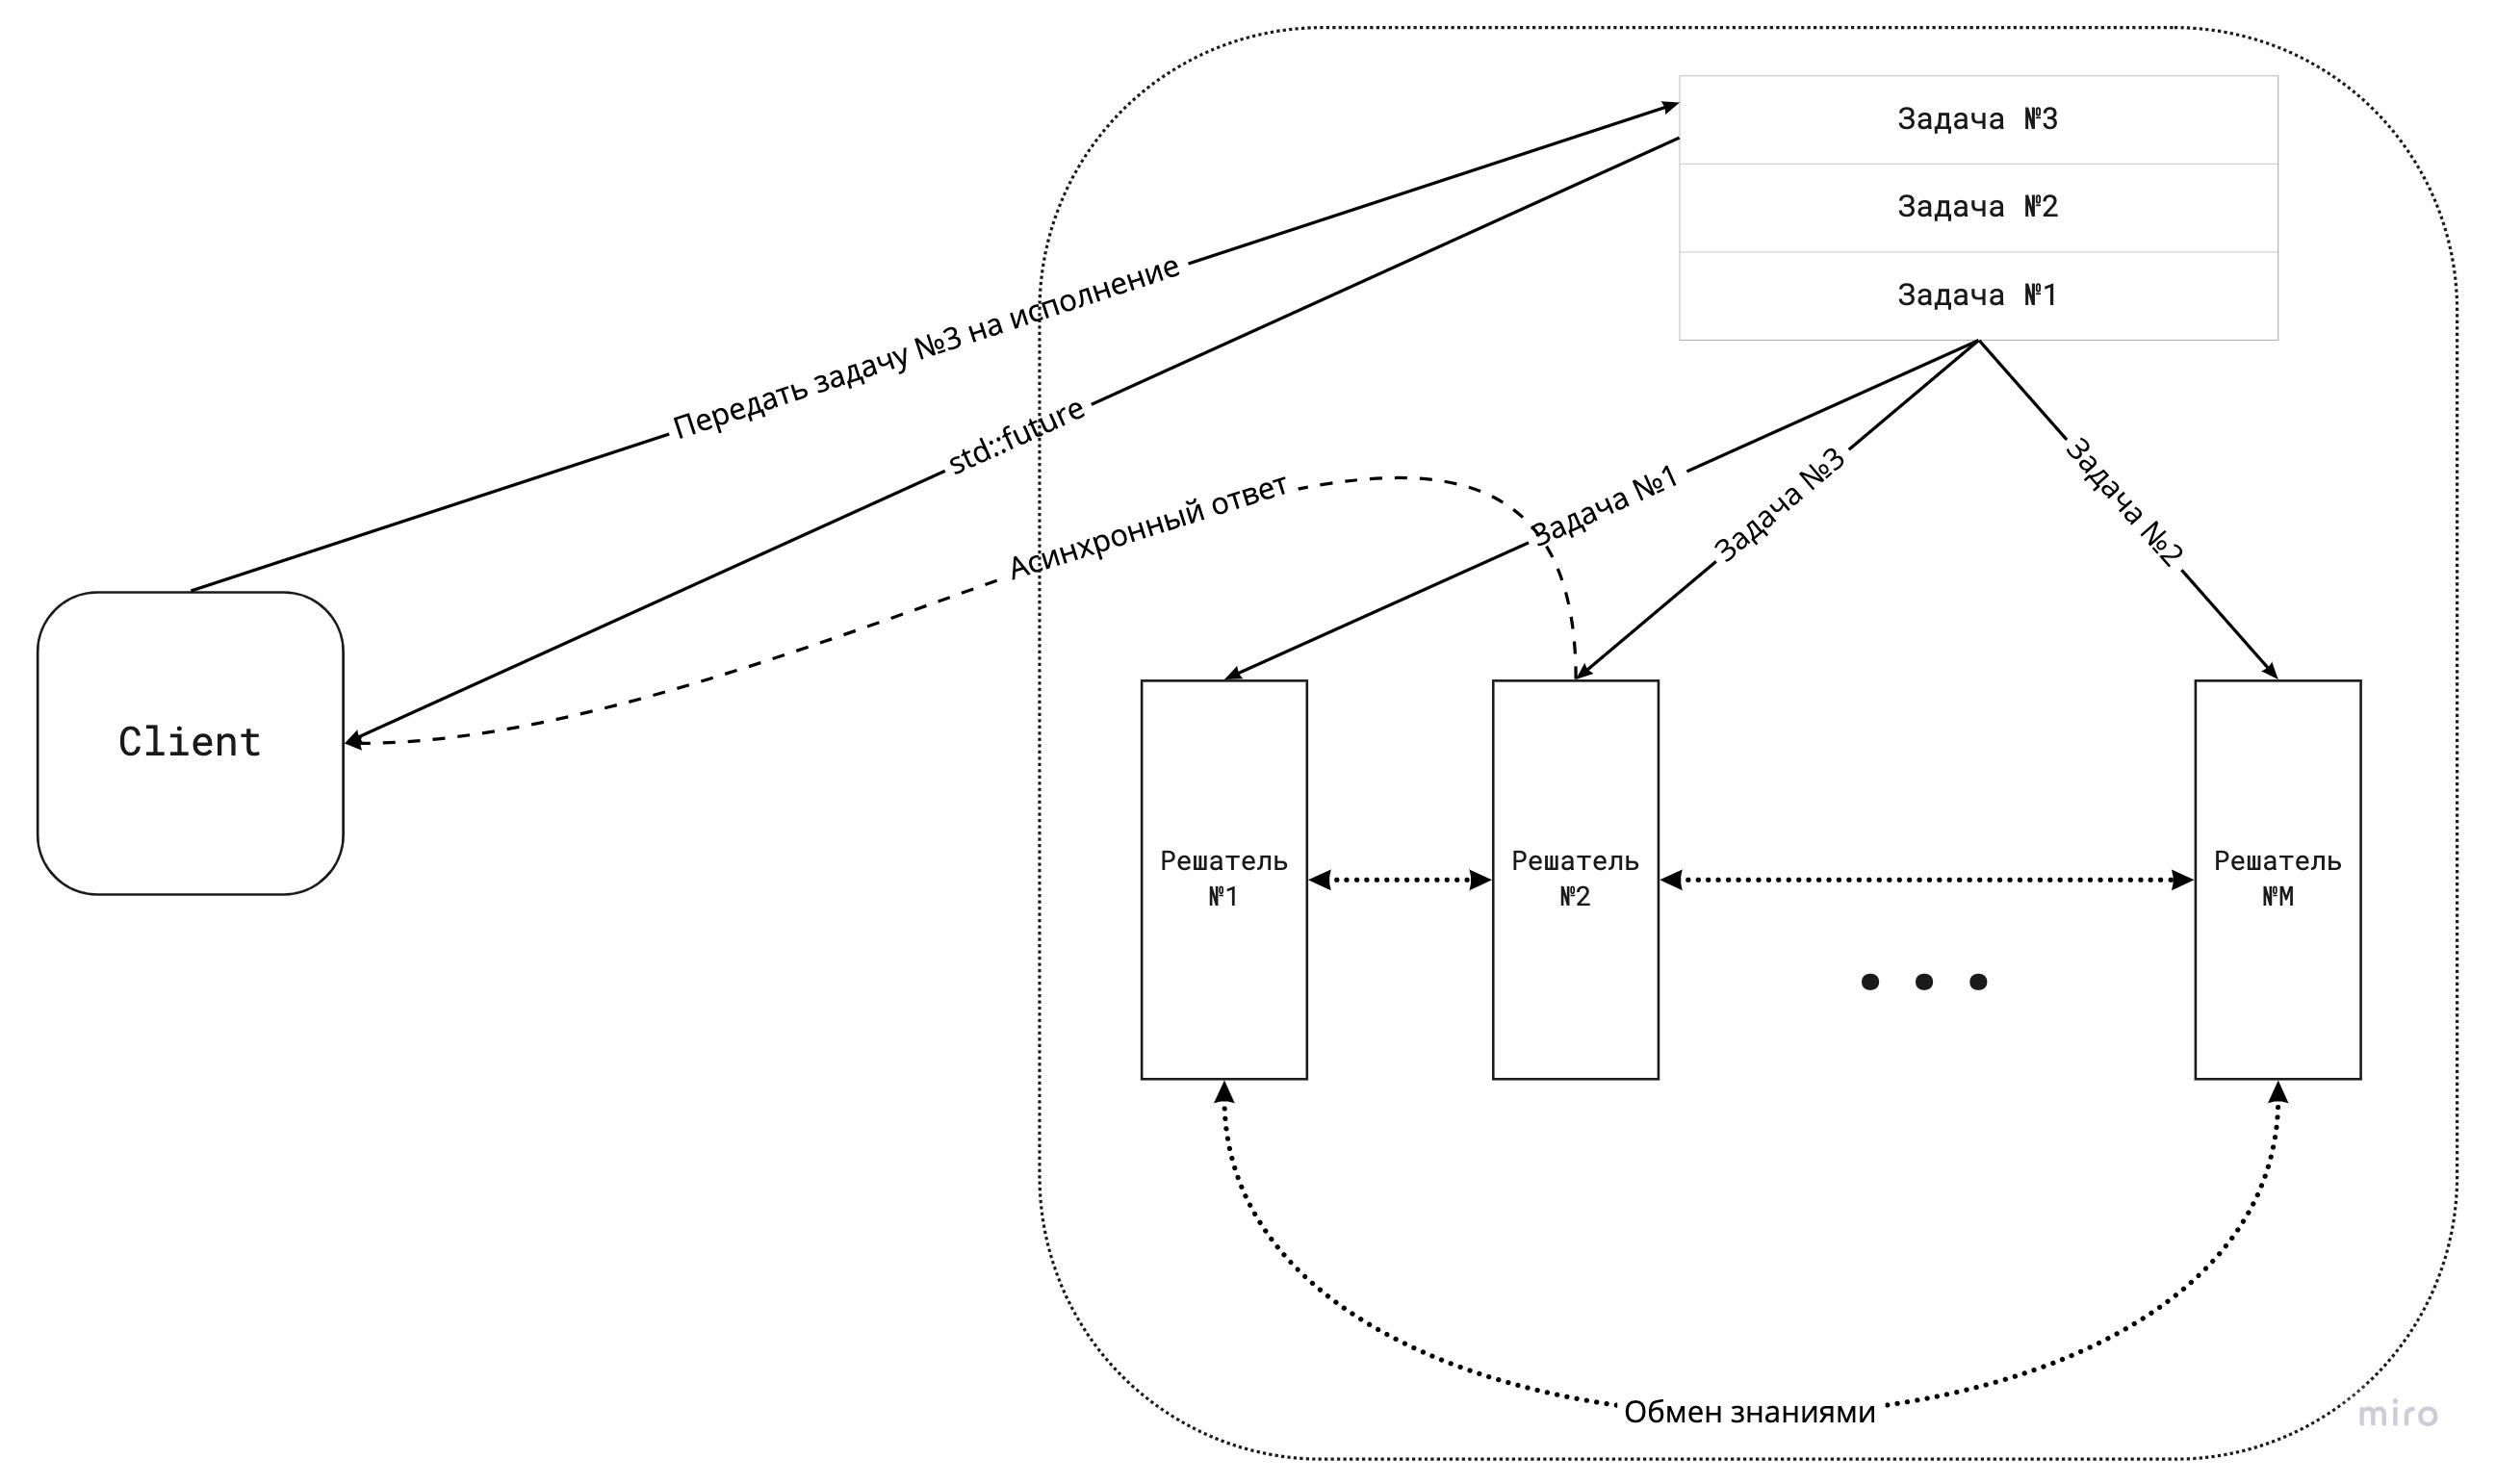
\includegraphics[width=\textwidth]{arch-seq}
    \label{arch:solver:seq-img}
\end{figure}

\section{Использование вероятностных лазеек}\label{arch:solve}

В данной главе описаны реализованные подходы к использованию вероятностных лазеек для решения
задач булевой выполнимости. Описаны \textit{прямой} и \textit{рекурсивный} подоходы к решению,
а также схема с \textit{использованием нескольких лазеек}.

\section{Описание реализации}\label{arch:impl}

В данной главе описана структура исходного кода алгоритма, перечислены возможные опции как при
сборке, так и при запуске приложения.

\chapterconclusion


\chapter{Практическое исследование}\label{research}

В данной главе описаны практические исследования, возникшие в процессе разработки алгоритма.
В разделе~\ref{research:prop} изложены эксперименты касательно эффективности предлагаемых
алгоритмов вывода последствий. В разделе~\ref{research:evol} --- эксперименты, касающиеся
эволюционных алгоритмов, описанных в разделе~\ref{arch:rbs:schema}. Также в разделе~\ref{research:final}
проведены замеры как базового решателя \textsc{painless-mcomsps}, так и разработанного в данной 
работе. Сделаны выводы о сильных и слабых сторонах полученного решения.

\section{Алгоритмы вывода последствий}\label{research:prop}

\section{Эволюционные алгоритмы}\label{research:evol}

\section{Оценка производительности решателя}\label{research:final}

\chapterconclusion

\tbd{Заключение}


\startconclusionpage



\printmainbibliography

\end{document}
